\subsubsection{Algoritmo de Kuhn (Emparelhamento Bipartido Máximo)}
O emparelhamento bipartido máximo (\textit{Maximum Bipartite Matching})
encontra o maior conjunto possível de arestas em um grafo bipartido onde
nenhuma aresta compartilha um vértice final. O Algoritmo de Kuhn resolve isso
utilizando caminhos de aumento via DFS de forma muito elegante. Complexidade:
$\mathcal{O}(V \cdot E)$.

\paragraph{Pseudo-Código: }\mbox{}\\
\begin{algorithm}[H]
    \SetAlgoLined
    \SetKwFunction{Kuhn}{try\_kuhn}
    \SetKwProg{Fn}{Função}{:}{}

    \Fn{\Kuhn{$v, adj, visitado, emparelhamento$}}{
        \If{$visitado[v]$}{
            \Retorna \text{falso}\;
        }
        $visitado[v] \gets \text{true}$\;
        \ParaCada{$to \in adj[v]$}{
            \Se{$emparelhamento[to] == -1$ \textbf{ou} \Kuhn{$emparelhamento[to], adj, visitado, emparelhamento$}}{
                $emparelhamento[to] \gets v$\;
                \Retorna \text{verdadeiro}\;
            }
        }
        \Retorna \text{falso}\;
    }
    \caption{Algoritmo de Kuhn para Emparelhamento Bipartido}
\end{algorithm}

Veja o Algoritmo de Kuhn encontrando o emparelhamento máximo:\\ \vspace{0.5cm}
\noindent
\begin{minipage}[t]{0.31\textwidth}
    \centering
    \textbf{Passo 1: Lados $L$ e $R$}\\
    \vspace{0.2cm}
    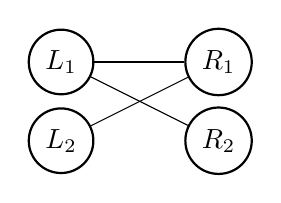
\begin{tikzpicture}[every node/.style={circle, draw, minimum size=0.5cm, thick}, >=stealth]
        \node (L1) at (0, 0.5) {$L_1$};
        \node (L2) at (0, -0.5) {$L_2$};
        \node (R1) at (2, 0.5) {$R_1$};
        \node (R2) at (2, -0.5) {$R_2$};
        \draw (L1) -- (R1);
        \draw (L1) -- (R2);
        \draw (L2) -- (R1);
    \end{tikzpicture}

    \vspace{0.2cm}
    \footnotesize
    \raggedright
    Grafo dividido em dois conjuntos disjuntos $L$ e $R$. Nenhum casamento inicial.
\end{minipage}%
\hfill
%
\begin{minipage}[t]{0.31\textwidth}
    \centering
    \textbf{Passo 2: Tentativa de Casamento}\\
    \vspace{0.2cm}
    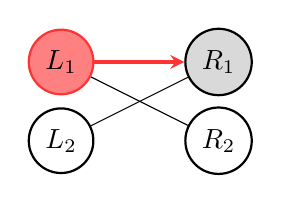
\begin{tikzpicture}[every node/.style={circle, draw, minimum size=0.5cm, thick}, >=stealth]
        \node[fill=red!50, draw=red!80] (L1) at (0, 0.5) {$L_1$};
        \node (L2) at (0, -0.5) {$L_2$};
        \node[fill=gray!30] (R1) at (2, 0.5) {$R_1$};
        \node (R2) at (2, -0.5) {$R_2$};
        \draw[->, very thick, red!80] (L1) -- (R1);
        \draw (L1) -- (R2);
        \draw (L2) -- (R1);
    \end{tikzpicture}

    \vspace{0.2cm}
    \footnotesize
    \raggedright
    $L_1$ tenta casar com $R_1$. Como $R_1$ está livre, o casamento é feito com sucesso.
\end{minipage}%
\hfill
%
\begin{minipage}[t]{0.31\textwidth}
    \centering
    \textbf{Passo 3: Caminho de Aumento}\\
    \vspace{0.2cm}
    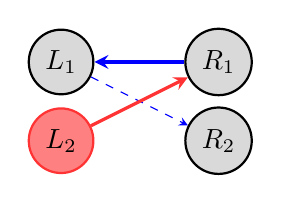
\begin{tikzpicture}[every node/.style={circle, draw, minimum size=0.5cm, thick}, >=stealth]
        \node[fill=gray!30] (L1) at (0, 0.5) {$L_1$};
        \node[fill=red!50, draw=red!80] (L2) at (0, -0.5) {$L_2$};
        \node[fill=gray!30] (R1) at (2, 0.5) {$R_1$};
        \node[fill=gray!30] (R2) at (2, -0.5) {$R_2$};
        \draw[->, dashed, blue] (L1) -- (R2);
        \draw[->, very thick, red!80] (L2) -- (R1);
        \draw[->, very thick, blue] (R1) -- (L1);
    \end{tikzpicture}

    \vspace{0.2cm}
    \footnotesize
    \raggedright
    $L_2$ quer $R_1$ (ocupado). $L_1$ muda para $R_2$, liberando $R_1$ para $L_2$!
\end{minipage}

\vspace{0.3cm}
\newpage
\paragraph{Implementação: }\mbox{}\\
\textbf{C++:}
\begin{lstlisting}[language=C++]
vector<vector<int>> adj;
vector<int> mt;
vector<bool> visited;

bool try_kuhn(int v) {
    if (visited[v]) return false;
    visited[v] = true;
    for (int to : adj[v]) {
        if (mt[to] == -1 || try_kuhn(mt[to])) {
            mt[to] = v;
            return true;
        }
    }
    return false;
}

int max_bipartite_matching(int n, int m) {
    //n = nos do lado esquerdo, m = nos do lado direito
    mt.assign(m, -1);
    int count = 0;
    for (int v = 0; v < n; ++v) {
        visited.assign(n, false);
        if (try_kuhn(v)) ++count;
    }
    return count;
}
\end{lstlisting}
\newpage